\chapter{Arhitektura i dizajn sustava}
		
		%\textbf{\textit{dio 1. revizije}}\\

		\textit{ Potrebno je opisati stil arhitekture te identificirati: podsustave, preslikavanje na radnu platformu, spremišta podataka, mrežne protokole, globalni upravljački tok i sklopovsko-programske zahtjeve. Po točkama razraditi i popratiti odgovarajućim skicama:}
	\begin{itemize}
		\item 	\textit{izbor arhitekture temeljem principa oblikovanja pokazanih na predavanjima (objasniti zašto ste baš odabrali takvu arhitekturu)}
		\item 	\textit{organizaciju sustava s najviše razine apstrakcije (npr. klijent-poslužitelj, baza podataka, datotečni sustav, grafičko sučelje)}
		\item 	\textit{organizaciju aplikacije (npr. slojevi frontend i backend, MVC arhitektura) }		
	\end{itemize}

	
		
	\pagebreak
		

				
		\section{Baza podataka}
			
			%\textbf{\textit{dio 1. revizije}}\\
			
		%\textit{Potrebno je opisati koju vrstu i implementaciju baze podataka ste odabrali, glavne komponente od kojih se sastoji i slično.}
		
		\textrm{Za naš sustav koristit ćemo relacijsku bazu podataka čija je struktura pogodna za modeliranje stvarnog svijeta. Gradivna jedinka baze je relacija, odnosno tablica koja je definirana svojim imenom i skupom atributa. Zadaća baze podataka je brza i jednostavna pohrana, izmjena i dohvat podataka za obradu. Baza podataka naše aplikacije sastoji se od sljedećih entiteta:}
		
	\begin{packed_item}
		
	\item Račun
	\item Posjetitelj
	\item Organizator
	\item Administrator
	\item Pretplata
	\item Plaćanje
	\item Događanje
	\item Interes
	\item Recenzija
	\item Media-Događanje
	\item Opcija-Obavijest
	\item Država
	\end{packed_item}
		
		
			\subsection{Opis tablica}
			

				%\textit{Svaku tablicu je potrebno opisati po zadanom predlošku. Lijevo se nalazi točno ime varijable u bazi podataka, u sredini se nalazi tip podataka, a desno se nalazi opis varijable. Svjetlozelenom bojom označite primarni ključ. Svjetlo plavom označite strani ključ}
				
				\textbf{Račun} \newline \textrm{ Ovaj entitet sadržava sve osnovne informacije o registriranom korisniku.
				Sadrži atribute: identifikator računa, korisničko ime, lozinka, e-mail, profilna slika, šifra država(ISO3), pripadna uloga.
				Ovaj entitet u vezi je \textit{One-to-One} s entitetima Posjetitelj, Organizator i Administrator preko atributa accountId i u vezi \textit{Many-to-One} s entitetom Država preko atributa countryCode.}
				\begin{longtblr}[
					label=none,
					entry=none
					]{
						width = \textwidth,
						colspec={|X[6,l]|X[6, l]|X[20, l]|}, 
						rowhead = 1,
					} %definicija širine tablice, širine stupaca, poravnanje i broja redaka naslova tablice
					\hline \SetCell[c=3]{c}{\textbf{Account}}	 \\ \hline[3pt]
					\SetCell{LightGreen}accountId & INT	&  	jedinstveni identifikator računa  	\\ \hline
					username	& VARCHAR &  jedinstveni identifikator korisnika 	\\ \hline 
					eMail & VARCHAR & E-Mail korisnika  \\ \hline 
					passwordHash & VARCHAR	&  	raspršeno kriptirana lozinka korisnika	\\ \hline 
					profileImage & VARCHAR	&  	lokalna adresa na profilnu sliku korisnika	\\ \hline 
					\SetCell{LightBlue}countryCode & CHAR(3)	&  	jedinstveni id države kojoj račun pripada u formatu 3 slova (Država.countryCode) 	\\ \hline
					roleId & INT	&  	šifra uloge pridružene korisniku	\\ \hline 
				\end{longtblr}
				
				
				
				\textbf{Posjetitelj} \newline \textrm{ Ovaj entitet specijalizacija je entiteta Račun namijenjena za "obične" korisnike.
					Sadrži atribute: identifikator računa, ime i prezime.
					Ovaj entitet u vezi je \textit{One-to-One} s entitetom Račun i u
					vezi \textit{One-to-Many} s entitetima Interes, Recenzija i Opcija-Obavijest preko atributa accountId.}
				\begin{longtblr}[
					label=none,
					entry=none
					]{
						width = \textwidth,
						colspec={|X[6,l]|X[6, l]|X[20, l]|}, 
						rowhead = 1,
					} %definicija širine tablice, širine stupaca, poravnanje i broja redaka naslova tablice
					\hline \SetCell[c=3]{c}{\textbf{Visitor}}	 \\ \hline[3pt]
					\SetCell{LightGreen}accountId & INT	&  	jedinstveni identifikator računa (Račun.accountId)  	\\ \hline
					firstName	& VARCHAR &  ime posjetitelja 	\\ \hline 
					lastName & VARCHAR & prezime posjetitelja  \\ \hline 
					
				\end{longtblr}
				
				\textbf{Organizator} \newline \textrm{ Ovaj entitet specijalizacija je entiteta Račun namijenjena za korisnike koji su organizatori.
					Sadrži atribute: identifikator računa, ime organizatora, vidljivost profila.
					Ovaj entitet u vezi je \textit{One-to-One} s entitetom Račun i u
					vezi \textit{One-to-Many} s entitetima s entitetima Plaćanje, Pretplata i Događanje preko atributa accountId.}
				\begin{longtblr}[
					label=none,
					entry=none
					]{
						width = \textwidth,
						colspec={|X[6,l]|X[6, l]|X[20, l]|}, 
						rowhead = 1,
					} %definicija širine tablice, širine stupaca, poravnanje i broja redaka naslova tablice
					\hline \SetCell[c=3]{c}{\textbf{Organizer}}	 \\ \hline[3pt]
					\SetCell{LightGreen}accountId & INT	&  	jedinstveni identifikator računa (Račun.accountId)   	\\ \hline
					organizerName	& VARCHAR &  naziv organizatora ili organizacije 	\\ \hline 
					hidden	& BOOLEAN &  zastavica koja govori o javnoj vidljivosti profila organizatora	\\ \hline 
					
					
				\end{longtblr}
				
				\textbf{Administrator} \newline \textrm{ Ovaj entitet specijalizacija je entiteta Račun namijenjena za korisnike koji su administratori.
					Sadrži atribute: identifikator računa.
					Ovaj entitet u vezi je \textit{One-to-One} s entitetom Račun preko atributa accountId.}
				\begin{longtblr}[
					label=none,
					entry=none
					]{
						width = \textwidth,
						colspec={|X[6,l]|X[6, l]|X[20, l]|}, 
						rowhead = 1,
					} %definicija širine tablice, širine stupaca, poravnanje i broja redaka naslova tablice
					\hline \SetCell[c=3]{c}{\textbf{Administrator}}	 \\ \hline[3pt]
					\SetCell{LightGreen}accountId & INT	&  	jedinstveni identifikator  računa (Račun.accountId) \\ \hline
					
				\end{longtblr}
				
				\textbf{Pretplata} \newline \textrm{ Ovaj entitet opisuje pretplatu koju je organizator nekad imao te koja može biti trenutno aktivna.
					Sadrži atribute: identifikator pretplate, datum početka pretplate, datum isteka pretplate, identifikator računa organizatora.
					Ovaj entitet u vezi je \textit{Many-to-One} s entitetom Organizator preko atributa accountId.}
				\begin{longtblr}[
					label=none,
					entry=none
					]{
						width = \textwidth,
						colspec={|X[6,l]|X[6, l]|X[20, l]|}, 
						rowhead = 1,
					} %definicija širine tablice, širine stupaca, poravnanje i broja redaka naslova tablice
					\hline \SetCell[c=3]{c}{\textbf{Subscription}}	 \\ \hline[3pt]
					\SetCell{LightGreen}subscriptionId & INT	&  	jedinstveni identifikator instance pretplate  	\\ \hline
					\SetCell{LightBlue}accountId & INT &  identifikator organizatora na kojeg se pretplata odnosi (Organizator.accountId) 	\\ \hline 
					startDate	& DATE &  datum početeka pretplate 	\\ \hline 
					expireDate	& DATE &  datum isteka pretplate 	\\ \hline 
				\end{longtblr}
				
				\textbf{Plaćanje} \newline \textrm{ Ovaj entitet opisuje plaćanje koje je organizator napravio prema našoj aplikaciji.
					Sadrži atribute: identifikator plaćanja, identifikator organizatora, datum plaćanja, iznos, metoda plaćanja.
					Ovaj entitet u vezi je \textit{Many-to-One} s entitetom Organizator preko atributa accountId.}
				\begin{longtblr}[
					label=none,
					entry=none
					]{
						width = \textwidth,
						colspec={|X[6,l]|X[6, l]|X[20, l]|}, 
						rowhead = 1,
					} %definicija širine tablice, širine stupaca, poravnanje i broja redaka naslova tablice
					\hline \SetCell[c=3]{c}{\textbf{Payment}}	 \\ \hline[3pt]
					\SetCell{LightGreen}paymentId & INT	&  	jedinstveni identifikator plaćanja 	\\ \hline
					\SetCell{LightBlue}accountId & INT &  identifikator organizatora na kojeg se plaćanje odnosi (Organizator.accountId) 	\\ \hline 
					date	& DATETIME &  datum i vrijeme plaćanja 	\\ \hline 
					amount	& FLOAT &  plaćen iznos 	\\ \hline 
					payment- Method	& VARCHAR &  način uplate 	\\ \hline 
				\end{longtblr}
				\textbf{Događanje} \newline \textrm{ Ovaj entitet opisuje događanje organizirano od strane organizatora.
					Sadrži atribute: identifikator događanja, identifikator organizatora, naziv, opis, državu, grad, lokaciju, datum i vrijeme, cijenu, naslovnu sliku događanja.
					Ovaj entitet u vezi je \textit{Many-to-One} s entitetom Organizator preko atributa accountId i s entitetom Država preko atributa countryCode, vezi \textit{One-to-Many} s entitetom Recenzija preko atributa eventId, vezi \textit{Many-to-Many} s entitetom Posjetitelj preko veze Interes i atributa eventId te u vezi \textit{One-to-Many} s entitetom Media-Događanje također preko atributa eventId.}
				\begin{longtblr}[
					label=none,
					entry=none
					]{
						width = \textwidth,
						colspec={|X[6,l]|X[6, l]|X[20, l]|}, 
						rowhead = 1,
					} %definicija širine tablice, širine stupaca, poravnanje i broja redaka naslova tablice
					\hline \SetCell[c=3]{c}{\textbf{Event}}	 \\ \hline[3pt]
					\SetCell{LightGreen}eventId & INT	&  	jedinstveni identifikator događanja 	\\ \hline
					\SetCell{LightBlue}accountId & INT &  identifikator organizatora koji organizira događanje (Organizator.accountId) 	\\ \hline 
					title	& VARCHAR &  naziv događanja 	\\ \hline 
					description	& VARCHAR &  opis događanja 	\\ \hline 
					price	& FLOAT &  cijena događanja 	\\ \hline 
					display- ImageSource	& VARCHAR &  lokalna adresa naslovne slike događanja 	\\ \hline 
					dateTime	& DATETIME &  vrijeme i datum događanja 	\\ \hline 
					countryCode	& CHAR(3) & šifra države u kojoj se događanje održava (Država.countryCode)	\\ \hline 
					city	& VARCHAR &  grad u kojem se događanje održava 	\\ \hline 
					location	& VARCHAR &  lokacija na kojoj se događanje održava	\\ \hline 
					price	& FLOAT &  cijena događanja 	\\ \hline 
				\end{longtblr}
				
					\textbf{Interes} \newline \textrm{ Ovaj entitet predstavlja \textit{Many-to-Many} vezu interesa od strane Posjetitelja prema Događanju.
					Sadrži atribute: identifikator događanja, identifikator računa posjetitelja, stupanj zainteresiranosti.
					Ovaj entitet u vezi je \textit{Many-to-One} s entitetima Posjetitelj i Događanje preko atributa accountId i eventId.}
				\begin{longtblr}[
					label=none,
					entry=none
					]{
						width = \textwidth,
						colspec={|X[6,l]|X[6, l]|X[20, l]|}, 
						rowhead = 1,
					} %definicija širine tablice, širine stupaca, poravnanje i broja redaka naslova tablice
					\hline \SetCell[c=3]{c}{\textbf{Interest}}	 \\ \hline[3pt]
					\SetCell{LightGreen}eventId & INT	&  	indetifikator događanja na koje se interes odnosi (Događanje.eventId)	\\ \hline
					\SetCell{LightGreen}accountId & INT &  identifikator posjetitelja na kojeg se interes odnosi (Posjetitelj.accountId) 	\\ \hline 
					degree- OfInterest	& VARCHAR &  stupanj interesa 	\\ \hline 
				\end{longtblr}
				
					\textbf{Recenzija} \newline \textrm{ Ovaj entitet modelira recenzije ostavljene od strane Posjetitelja za pojedina Događanja.
					Sadrži atribute: jedinstveni identifikator recenzije, identifikator događanja, identifikator računa posjetitelja, komentar, datum, vrijeme.
					Ovaj entitet u vezi je \textit{Many-to-One} s entitetima Događanje i Posjetitelj preko atributa eventId i accountId.}
				\begin{longtblr}[
					label=none,
					entry=none
					]{
						width = \textwidth,
						colspec={|X[6,l]|X[6, l]|X[20, l]|}, 
						rowhead = 1,
					} %definicija širine tablice, širine stupaca, poravnanje i broja redaka naslova tablice
					\hline \SetCell[c=3]{c}{\textbf{Review}}	 \\ \hline[3pt]
					\SetCell{LightGreen}reviewId & INT	&  	jedinstveni identifikator ostavljene recenzije	\\ \hline
					\SetCell{LightBlue}accountId & INT &  identifikator posjetitelja koji je ostavio recenziju (Posjetitelj.accountId) 	\\ \hline 
					\SetCell{LightBlue}eventId	& INT &  identifikator događanja na koje se recenzija odnosi (Događanje.eventId) 	\\ \hline 
					comment	& VARCHAR &  ostavljen komentar 	\\ \hline 
					dateTime	& DATETIME &  vrijeme i datum ostavljene recenzije 	\\ \hline 
				\end{longtblr}
				
				
				
					\textbf{Media-Događanje} \newline \textrm{ Ovaj entitet sprema lokalne adrese foto i video sadržaja koje pripada događanju.
					Sadrži atribute: jedinstveni identifikator recenzije, identifikator događanja, identifikator računa posjetitelja, komentar, datum, vrijeme.
					Ovaj entitet u vezi je \textit{Many-to-One} s entitetima Događanje i Posjetitelj preko atributa eventId i accountId.}
				\begin{longtblr}[
					label=none,
					entry=none
					]{
						width = \textwidth,
						colspec={|X[6,l]|X[6, l]|X[20, l]|}, 
						rowhead = 1,
					} %definicija širine tablice, širine stupaca, poravnanje i broja redaka naslova tablice
					\hline \SetCell[c=3]{c}{\textbf{EventMedia}}	 \\ \hline[3pt]
					\SetCell{LightGreen}mediaId & INT	&  	jedinstveni identifikator materijala	\\ \hline
					\SetCell{LightBlue}eventId	& INT &  identifikator događanja na koje se materijal odnosi (Događanje.eventId) 	\\ \hline 
					mediaType	& VARCHAR &  vrsta sadrđaja; slika ili video 	\\ \hline 
					mediaSource	& VARCHAR &  lokalna adresa sadržaja	\\ \hline 
				\end{longtblr}
				
					\textbf{Opcija-Obavijest} \newline \textrm{ Ovaj entitet sprema informaciju o tome koji korisnik ima aktiviran koji način slanja obavijesti.
					Sadrži atribute: identifikator posjetitelja, vrsta obavijesti.
					Ovaj entitet u vezi je \textit{Many-to-One} s entitetom Posjetitelj preko atributa accountId.}
				\begin{longtblr}[
					label=none,
					entry=none
					]{
						width = \textwidth,
						colspec={|X[6,l]|X[6, l]|X[20, l]|}, 
						rowhead = 1,
					} %definicija širine tablice, širine stupaca, poravnanje i broja redaka naslova tablice
					\hline \SetCell[c=3]{c}{\textbf{NotificationOption}}	 \\ \hline[3pt]
					\SetCell{LightGreen}accountId & INT	&  	jedinstveni identifikator posjetitelja (Posjetitelj.accountId)	\\ \hline
					\SetCell{LightGreen}type & VARCHAR	&  	vrsta obavijesti. (Primarni ključ je uređeni par accountId, type)	\\ \hline
				\end{longtblr}
				
				
					\textbf{Država} \newline \textrm{ Ovaj entitet modelira državu sa pripadnim šiframa i nazivom države.
					Sadrži atribute: identifikator države, sekundarni identifikator države, ime države.
					Ovaj entitet u vezi je \textit{One-to-Many} s entitetima Događanje i račun preko atributa countryCode.}
				\begin{longtblr}[
					label=none,
					entry=none
					]{
						width = \textwidth,
						colspec={|X[6,l]|X[6, l]|X[20, l]|}, 
						rowhead = 1,
					} %definicija širine tablice, širine stupaca, poravnanje i broja redaka naslova tablice
					\hline \SetCell[c=3]{c}{\textbf{Country}}	 \\ \hline[3pt]
					\SetCell{LightGreen}countryCode & CHAR(3)	&  	jedinstveni identifikator države sastavljen od 3 slova	\\ \hline
					code & CHAR(2)	&  	sekundarni jedinstveni identifikator države sastavljen od 2 slova	\\ \hline
					name & VARCHAR	&  	naziv države	\\ \hline
				\end{longtblr}
				
				
			\subsection{Dijagram baze podataka}
				%\textit{ U ovom potpoglavlju potrebno je umetnuti dijagram baze podataka. Primarni i strani ključevi moraju biti označeni, a tablice povezane. Bazu podataka je potrebno normalizirati. Podsjetite se kolegija "Baze podataka".}
				
				\begin{figure}[htbp]
					\centering
					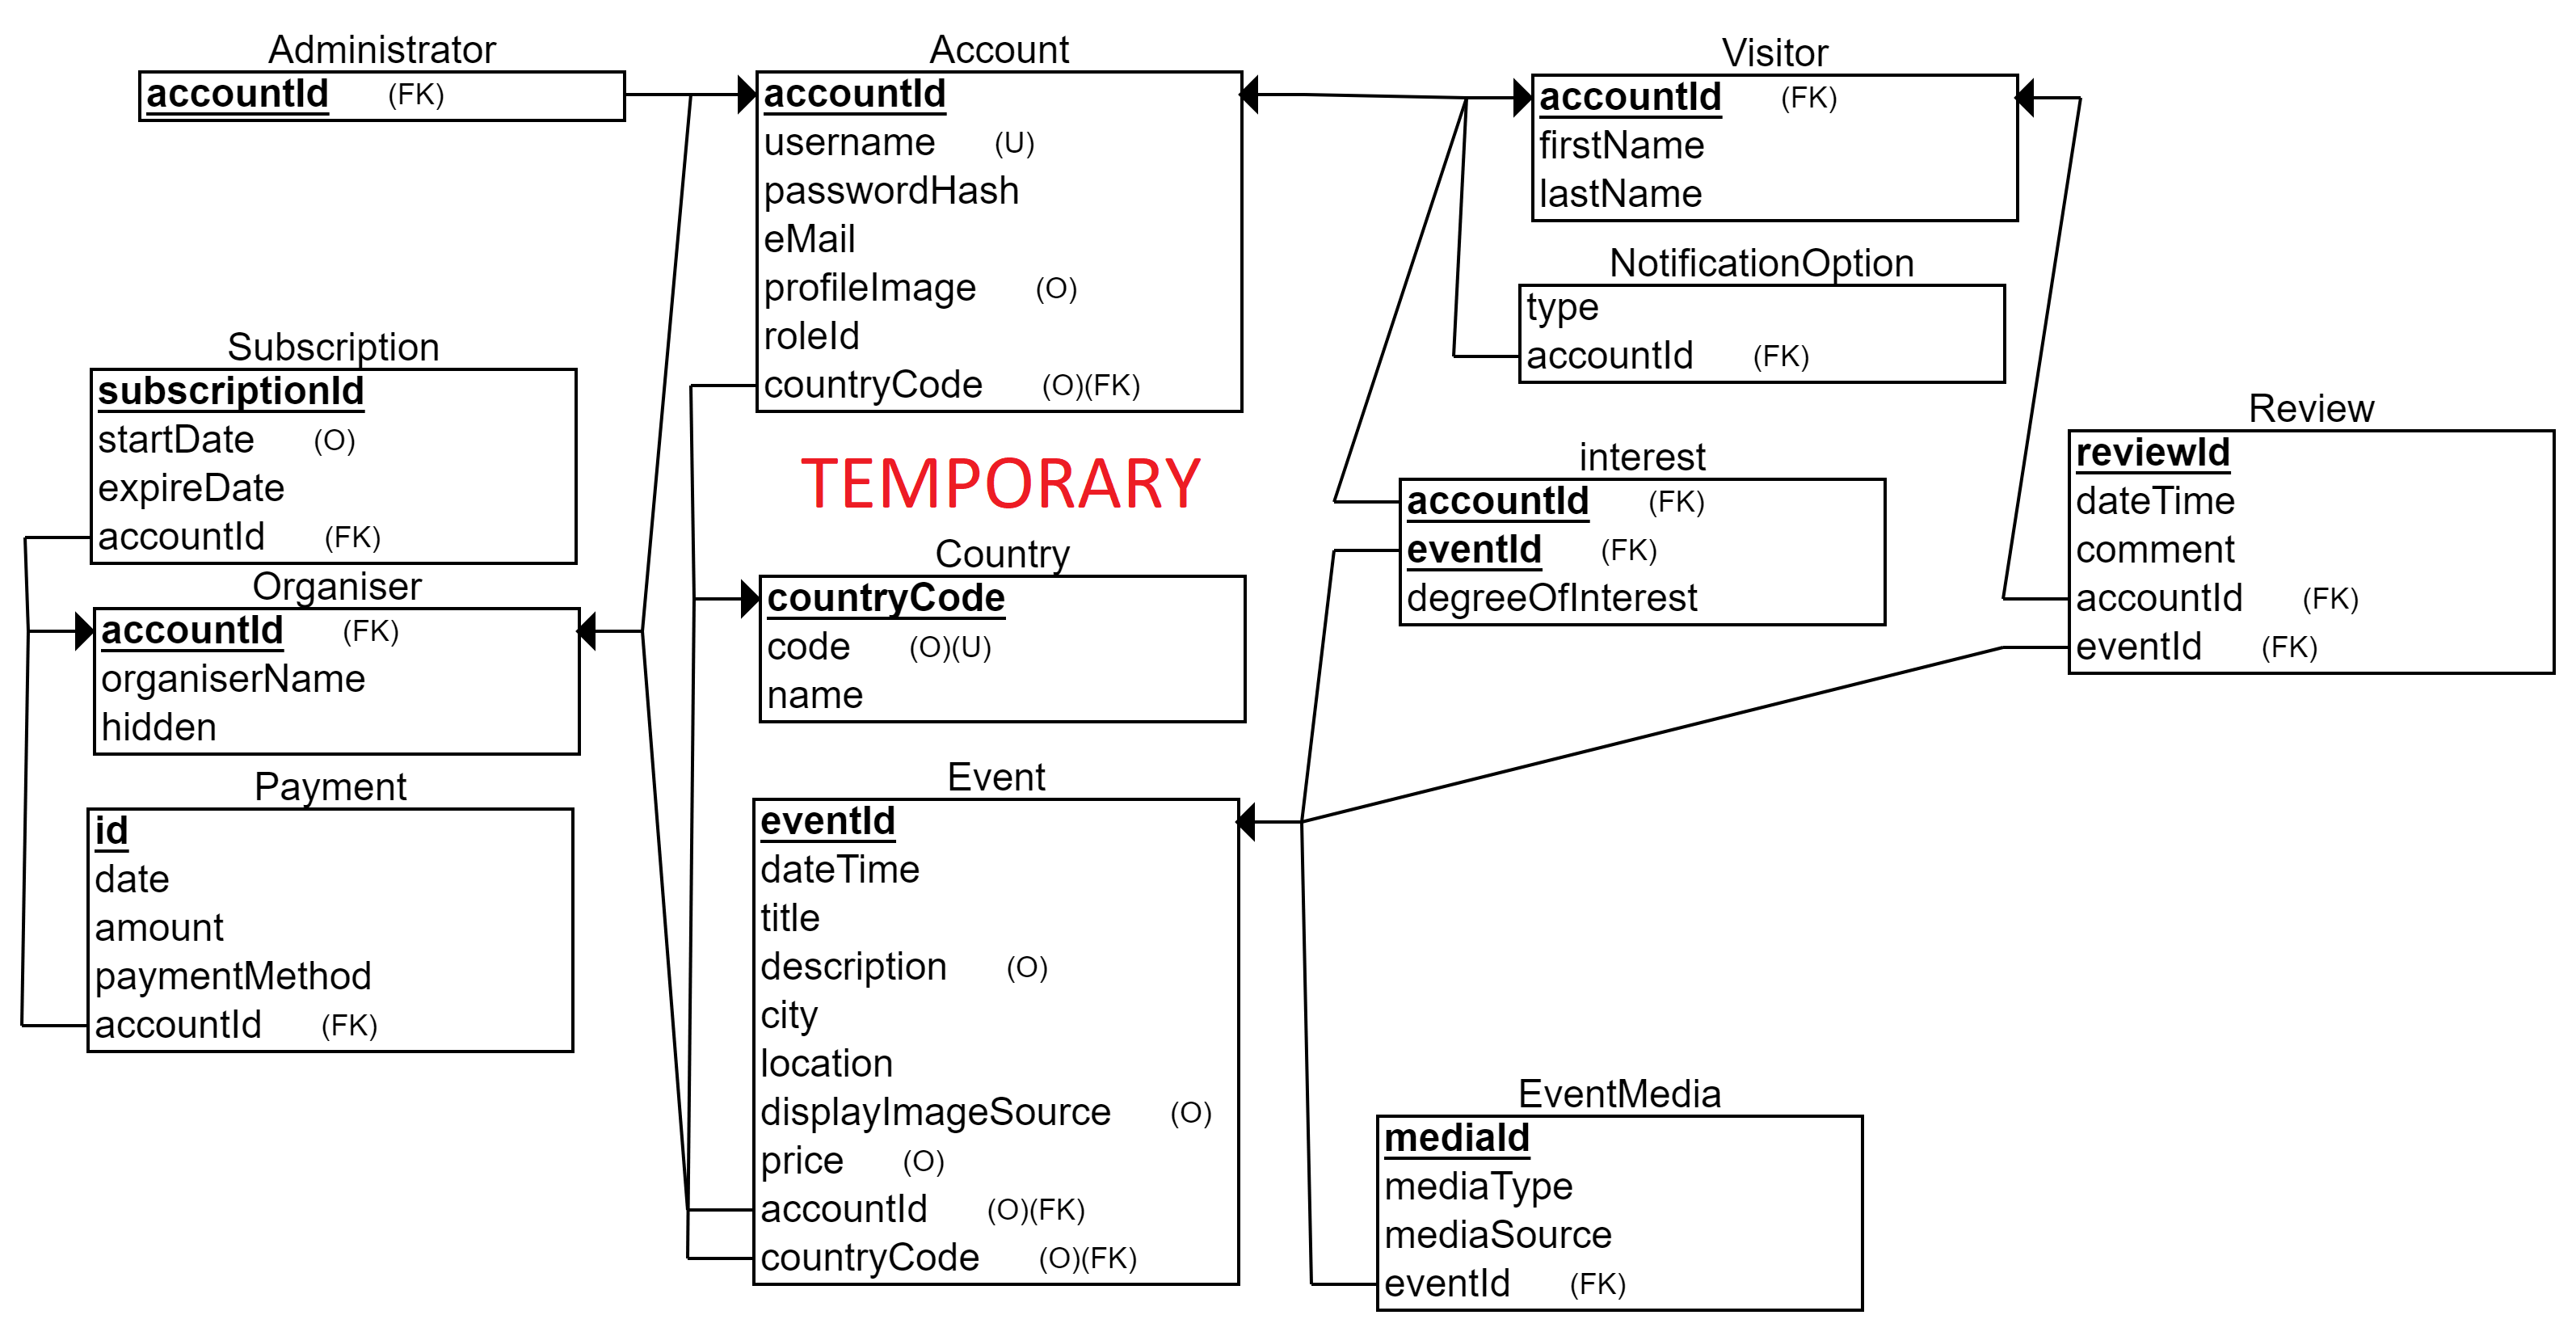
\includegraphics[width=1\textwidth]{dijagrami/rel_dijagram.png}
					\caption{Relacijski dijagram baze podataka}
					\label{fig:my_image}
				\end{figure}
				
				
	
			\eject
			
			
		\section{Dijagram razreda}
		
			\textit{Potrebno je priložiti dijagram razreda s pripadajućim opisom. Zbog preglednosti je moguće dijagram razlomiti na više njih, ali moraju biti grupirani prema sličnim razinama apstrakcije i srodnim funkcionalnostima.}\\
			
			\textbf{\textit{dio 1. revizije}}\\
			
			\textit{Prilikom prve predaje projekta, potrebno je priložiti potpuno razrađen dijagram razreda vezan uz \textbf{generičku funkcionalnost} sustava. Ostale funkcionalnosti trebaju biti idejno razrađene u dijagramu sa sljedećim komponentama: nazivi razreda, nazivi metoda i vrste pristupa metodama (npr. javni, zaštićeni), nazivi atributa razreda, veze i odnosi između razreda.}\\
			
			\textbf{\textit{dio 2. revizije}}\\			
			
			\textit{Prilikom druge predaje projekta dijagram razreda i opisi moraju odgovarati stvarnom stanju implementacije}
			
			
			
			\eject
		
		\section{Dijagram stanja}
			
			
			\textbf{\textit{dio 2. revizije}}\\
			
			\textit{Potrebno je priložiti dijagram stanja i opisati ga. Dovoljan je jedan dijagram stanja koji prikazuje \textbf{značajan dio funkcionalnosti} sustava. Na primjer, stanja korisničkog sučelja i tijek korištenja neke ključne funkcionalnosti jesu značajan dio sustava, a registracija i prijava nisu. }
			
			
			\eject 
		
		\section{Dijagram aktivnosti}
			
			\textbf{\textit{dio 2. revizije}}\\
			
			 \textit{Potrebno je priložiti dijagram aktivnosti s pripadajućim opisom. Dijagram aktivnosti treba prikazivati značajan dio sustava.}
			
			\eject
		\section{Dijagram komponenti}
		
			\textbf{\textit{dio 2. revizije}}\\
		
			 \textit{Potrebno je priložiti dijagram komponenti s pripadajućim opisom. Dijagram komponenti treba prikazivati strukturu cijele aplikacije.}